\documentclass[aip,pop,amsmath,amssymb,reprint,superscriptaddress]{revtex4-1} %preprint version
\usepackage{graphicx}% Include figure files
\usepackage{dcolumn}% Align table columns on decimal point
\usepackage{bm}% bold math

    \renewcommand{\topfraction}{0.9}    % max fraction of floats at top
    \renewcommand{\bottomfraction}{0.8}    % max fraction of floats at bottom
    \setcounter{topnumber}{2}
    \setcounter{bottomnumber}{2}
    \setcounter{totalnumber}{4}     % 2 may work better
    \setcounter{dbltopnumber}{2}    % for 2-column pages
    \renewcommand{\dbltopfraction}{0.9}    % fit big float above 2-col. text
    \renewcommand{\textfraction}{0.07}    % allow minimal text w. figs
    \renewcommand{\floatpagefraction}{0.7}    % require fuller float pages
    \renewcommand{\dblfloatpagefraction}{0.7}    % require fuller float pages
    \setlength{\abovecaptionskip}{5pt}
    \setlength{\belowcaptionskip}{5pt}
    \setlength{\parskip}{0pt}
    \setlength{\textfloatsep}{5pt} 

\begin{document}
\title{Obseravation a coherent Drift-Rotational modes with Strong Driven Rotation on the Large Plasma Device}
\author{D.A. Schaffner}
\author{T.A Carter}
\author{G.D. Rossi}
\author{D.S. Guice}
\author{J.E. Maggs}
\author{S. Vincena}
\author{B. Friedman}
\affiliation{Department of Physics and Astronomy, University of California, Los Angeles}
\date{\today}
\begin{abstract}
The instabilities observed on the Large Plasma Device (LAPD) [W. Gekelman, \textit{et. al}, Rev. Sci. Instr. \textbf{62}, 2875 (1991)] are explored in conjunction with a the ability to finely adjust azimuthal flow and flow shear.

\end{abstract}
\maketitle

\section{Introduction}

The nature of the types of instabilities found in the LAPD plasmas can have important effects on the resulting turbulence and transport. One example of this effect is in the scaling of turbulence and transport suppression with shear as discussed in the variations of decorrelation models of shear suppression which make different assumptions on the instabilities present and driving the turbulence~\cite{schaffner13}. Instability identification in a turbulent setting can be an extremely difficult task as there are many simultaneous sources of free energy as well as the fact that non-linear fluctuation behavior can be vastly different than the linear modes that might originate it. Nevertheless, mode identification (or at least categorization) can be useful in understanding the physical mechanisms in turbulence and transport so any attempt is worthy.

This biasing experiment in LAPD provides a useful approach to mode identification as it has been shown that biasing can significantly modify the plasma gradients present thus changing the drive of different linear instabilities. The three main linear instabilities that will be analyzed in this section are the resistive drift-wave (hereafter DW), the rotational interchange mode (RI), and the Kelvin-Helmholtz instability (KH). The resistive pressure-gradient driven instability or drift-wave has been shown to be present in the LAPD in~\cite{penano00}. Investigations and identification of the KH mode was made on the LAPD in~\cite{horton04,perez06}. Linear calculations using a Braginskii fluid model (discussed later in the section) has shown that given experimental profiles---those taken from previous biasing experiments on LAPD~\cite{maggs07,carter09}---the activity of all three of these instabilities are present and the growth rates for all three modes are comparable~\cite{popovich10}. 

Simulations of LAPD turbulence using the BOUT++ code have revealed the presence of a nonlinear instability which overtakes the linear modes in establishing the resulting turbulent state~\cite{friedman12}. Thus it is possible that linear modes do not have any connection to the turbulent state in LAPD.  It should be noted however, that simulations have only been performed for the "null flow" state and that linear instabilities may explain the fluctuation spectrum (in particular the coherent mode) at higher biases.

Since the experimental data is taken from the steady-state portion of the plasma discharge, when growing linear instabilities will not only have already saturated, but will likely have already non-linearly interacted to form a broadband turbulent state, mode identification cannot rely entirely on the clues from the fluctuation and spectral data. The spectral information is combined with examination of location and strength of gradients which can drive the instabilities, the direction of propagation of these modes and comparison to the growth rates and frequencies of linear modes as calculated using a Braginskii fluid equation eigenfunction solver to narrow down the likelihood of contributions to the turbulence due to each of the three instabilities. The appearance of a distinct coherent mode in the highest biases is also helpful in distinguishing between mode types especially when compared to linear growth rates. While a full 3D non-linear simulation like BOUT++ can provide much better comparisons, the combination of the approaches mentioned can be highly suggestive.

The varying features of the spectral density functions---calculated using the two-point correlation technique---are used to distinguish amongst modes. By calculating the spectral density for different regions and different groupings of bias states, the features can be used to compare to both radial and bias locations of driving gradients as well as to growth rates from linear calculations restricted to similar spatial regions and bias groupings.

\section{Wavenumber-Frequency Spectral Density}

In addition to temporal fluctuation spectra, spatial spectra can be used to analyze turbulent properties of the plasma. The most accurate way to determine a spatial spectrum---that is, the distribution of fluctuation power broken into spatial eigenmodes---would be to have a simultaneous measurement of plasma parameters ($I_{\text sat}$,$V_{f}$) at a high resolution of multiple positions. While this can be partly achieved using multiple tipped Langmuir probes (such as the rake probe described in Chapter 3), such a probe offers far too little spatial resolution to be of very much use.  Instead, the high temporal resolution available to the Langmuir probe signals can be used to approximate a local wavenumber spectrum using a two-point correlation technique. This method uses the time correlation between two points to measure a relative phase, and with a known separation distance, a local wavenumber, $k_{l} = \theta/d$. Given a large enough number of statistics, a distribution of local wavenumber as a function of frequency and position can be created. The details of this process are discussed in detail in Appendix B. The results of such an analysis yield spectral density functions which is a histogram of fluctuation power binned by wavenumber and frequency. 

Since the LAPD is a cylindrical device, it is most natural to cast eigenmodes of the system with as having an azimuthal component $\sim e^{im \theta}$ with mode number, m; an axial component $\sim e^{inz}$, with eigenvalue n; and a radial eigenfunction \textit{f}(r). The stability of the relevant modes depend most on the azimuthal mode number, m, (and consequently the resulting transport)and is thus of most interest for turbulence study. Though m-numbers are the more physically relevant quantity, the two-point correlation method used here determines an azimuthal wavenumber first, where $k_{\theta} = m/r$. The results will be shown first cast in terms of $k_{\theta}$ and a frequently used ratio, $k_{\theta}\rho_{s}$, but will also be shown in terms of azimuthal mode numbers.

\begin{figure}[!htbp]
\centerline{
\includegraphics[width=8.5cm]{k_spec_byBias_lab.png}}
\caption{\label{fig:k_spec_byBias_lab} Perp Wavenumber spectra for four  different bias groups (a)Low/Unbiased IDD flow Bias0-2, (b)Min Flow Bias10-12 (c)Low EDD Flow Bias 16-18 and (d)Strong EDD flow Bias 25-27.}
\end{figure}

The global changes in power frequency and wavenumber space as a function of bias can be seen in Figure~\ref{fig:k_spec_byBias_lab}. The spectral amplitude is histograms into bins 312Hz wide in frequency, and 0.01 $\text{cm}^{-1}$ wide in wavenumber space. Spectral density histogram (a) is averaged over all radial locations from 12-32cm and over Bias 0,1, and 2, which are essentially all unbiased cases (they are all biases less than the floating potential). Histogram (b) shows the average of three biases around where the plasma rotation nulls out---Bias 10,11 and 12. Histogram (c) averages biases in the low to medium EDD flow regime---Bias 16,17, and 18. Finally, Histogram (d) averages some strong EDD flow biases---Bias 25,26 and 27. 

As with the line plots above, these spectral density functions show the overall shift in propagation direction for the modes as the bias is increased. These plots show that the vast majority of the fluctuation power resides in the frequency space less than 10kHz and within a wavenumber space less than 2.0 $\text{cm}^{-1}$ or, assuming an ion sound radius of $\rho_{s} \sim 0.5$cm, within a $k_{\perp}\rho_{s} < 1$. Power does expand out into a narrow band that increases approximately linearly in both frequency and wavenumber. In the unbiased state, a line fit along this strip would have a slope that corresponded to a phase velocity, $v_{p} = f/k = 2 \times 10^{4} $cm/s which is about an order of magnitude less than the peak flows observed in this state. This confirms that these distributions are not set entirely by the Doppler shift.

As the bias is increased to the point where plasma rotation minimized, fluctuation amplitude begins to be concentrated toward smaller wavenumber and frequency. Both the frequency and wavenumber of the linear feature in the IDD direction decreases and its slope decreases slightly to a phase velocity of $1.5 \times 10^{4}$ cm/s which shows the slight impact of Doppler shifting on phase velocity. There is also slightly more power in the EDD direction. It should be noted, though that even in the minimum flow state, there is still moderate amounts of flow in the IDD at the far edge or $r>30$cm as can be seen in Figure~\ref{fig:velocity_profiles}. In fact, the far edge flow appears to be consistently in the IDD beyond 30cm even for the flow states with the highest peak driven flow. This can be seen in these four plots by the presence of power in the IDD which is never completely eliminated. 

For biases that cause plasma to rotate a low to medium rates in the EDD direction, as in Figure~\ref{fig:k_spec_byBias}(c), there is a clear difference in distribution for modes that propagate in the EDD and those still propagating in the IDD. The IDD modes maintain the narrow lobe shape that is reminiscent of the unbiased case and can somewhat still be fit by a linear dispersion relation with phase velocity on the order of $\sim 1.5-2 \times 10^{4}$ cm/s. The EDD modes on the other hand are more broadly distributed in the range from 0-40kHz and 0-4 $\text{cm}^{-1}$. No dispersion relation can be approximated in this region. This difference is perhaps an indication of differing origins of the turbulence and evidence that the biasing is changing the free energy drive of the turbulent fluctuations. 

The highest measured biases show the most significant change in the spectral distribution showing both the coherent mode at approximately f=10kHz and k=0.5$\text{cm}^{-1}$, but also fluctuation power in modes propagating predominantly in the EDD direction. Rather than being diffuse, a narrow lobe is formed like in the unbiased state, but with a steeper slope. An approximate fit to this slope yields a phase velocity more like $v_{p} \sim 4 \times 10^{4}$ cm/s. This could be due to a change in the underlying instability drive and resulting mode, or from the influence of the stronger EDD rotation in this state. Nevertheless, there is a clear transition in the nature of the turbulence not only from the unbiased state to the high biased, high rotation state, but even between the lower EDD rotation and higher EDD rotation states as in Figure~\ref{fig:k_spec_byBias}(c) and (d).

\section{Observation of Coherent Modes}

Fluctuation data from a recently conducted study of finely controlled azimuthal rotation on the LAPD~\cite{schaffner12} shows the emergence of a coherent mode with increasing limiter bias and thus azimuthal flow.

\begin{figure}[!htbp]
\centerline{
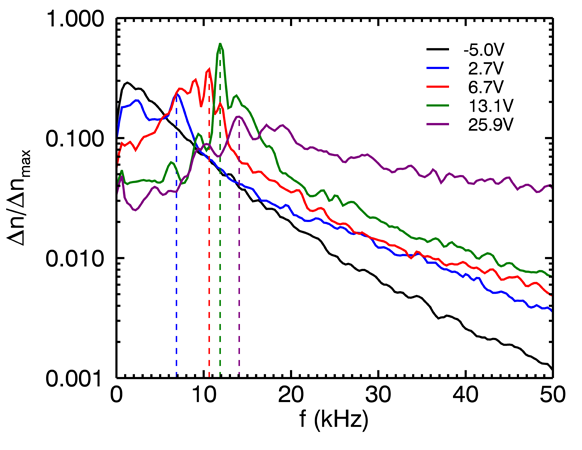
\includegraphics[width=8.5cm]{dens_spec_limedge_zoom.png}}% made using plot_density_spectra_mode_zoom_highbias.pro
\caption{\label{fig:dens_spec_limedge_zoom} Coherent modes for various biases}
\end{figure}

Figure~\ref{fig:dens_spec_limedge_zoom} shows the frequency spectra for various biases for frequencies up to 50kHz and focused in the region right around the limiter edge, where the presense of the coherent mode is strongest. Compared to the minimum flow case (Limiter-Anode = -5.0V), where the fluctuation spectrum is broadband, a clear peaks in the spectra emerge starting at a Limiter-Anode voltage difference of 2.7V and increasing in power and frequency up to a voltage difference of 13.1V. The highest bias listed, with a voltage difference of 25.9V, shows a reduction in power and less distinct peaks.

The mode is shown to be highly localized at the limiter edge.

\begin{figure}[!htbp]
\centerline{
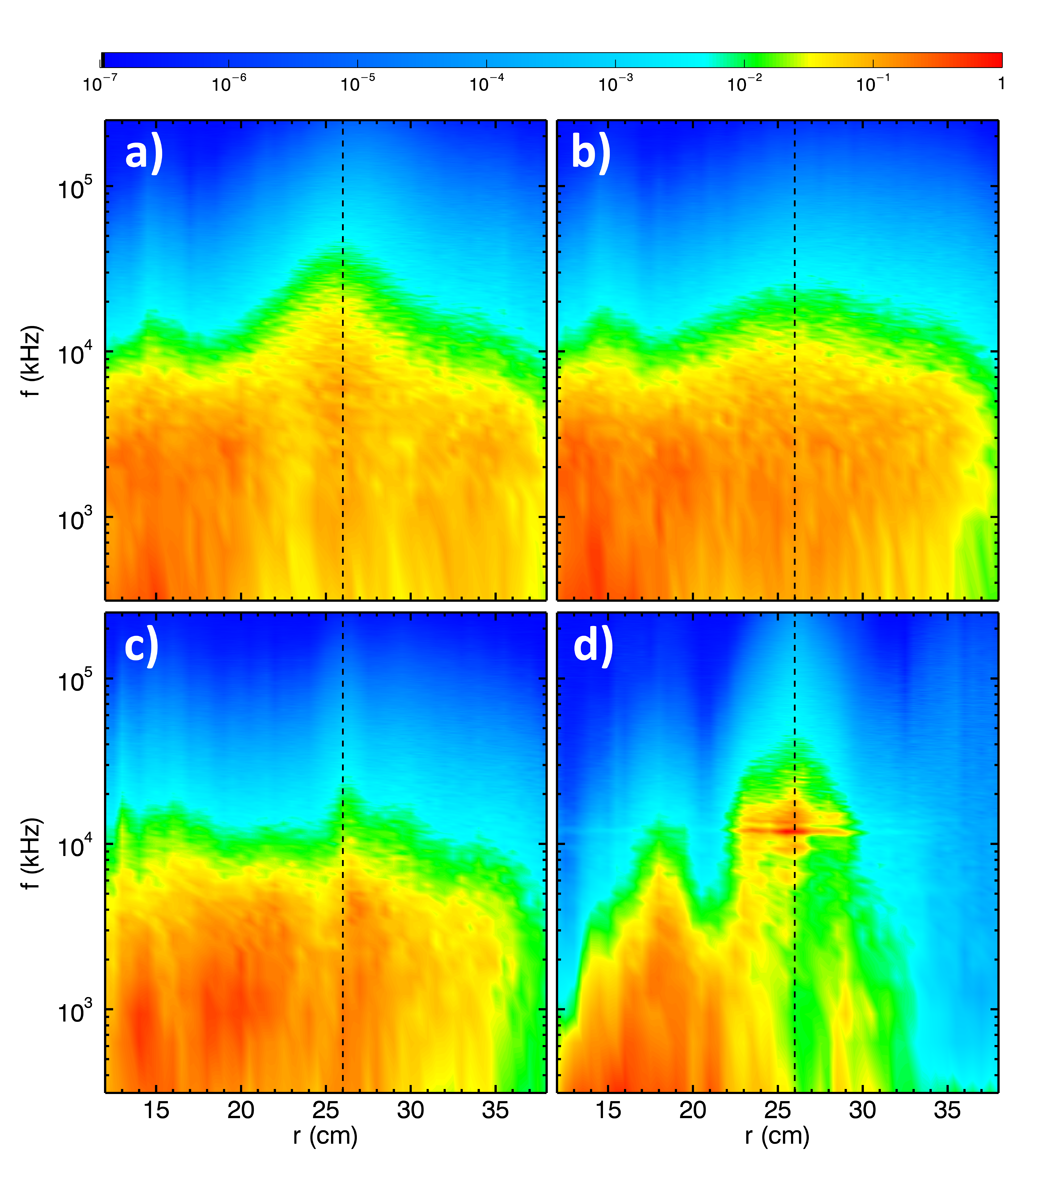
\includegraphics[width=8.5cm]{dens_spec_contours_4bias_lab}}% made %using plot_density_spectra_contours_byBias.pro
\caption{\label{fig:dens_spec_contours_4bias} Contour Plots of Density fluctuation power (normalized to the maximum value) versus frequency and radius for (a)0bias, (b)Bias 7, (c)Bias18, (d)Bias27}
\end{figure}

Figure~\ref{fig:dens_spec_contours_4bias} shows the spatial distribution of turbulent fluctuations for four different biases: (a) an unbiased state with small IDD flow, (b) a minimum shearing state, (c)a small EDD flow, and (d) a strong EDD flow state. Each of the four contour plots show the logarithm of the density fluctuation power as a function of both radius and frequency with the limiter edge indicated by the dashed line at 26cm. All four plots are normalized to the same maximum fluctuation value. In the first plot, (a), the fluctuation power is generally fairly evenly distributed radially. As mentioned before, most of the fluctuation power is concentrated in the band $<10kHz$. There is a slight spreading of power in frequency at the limiter edge. This could be due partially to Doppler shifting of the frequency from the spontaneous flow, though the peak flow in this stage occurs at about 28cm. There is also a local maximum of fluctuation amplitude at the limiter edge. 

Though the previous spectral distribution plots showed that the core region usually had a smaller amount of fluctuation power overall, in this very low frequency regime, the core region tends to have the highest absolute fluctuation amplitude. Evidence for this trend was also observed in the fluctuation profiles as in Figure~\ref{fig:dens_flucs_profs}. However, as that same figure shows, it is clear that the core region generally has the lowest percentage fluctuation amplitude when compared to the density level. 

Figures~\ref{fig:dens_spec_contours_4bias}(b) and ~\ref{fig:dens_spec_contours_4bias}(c) show the modification of the spatial distribution as the limiter bias is increased to -6.3V below the anode(b) and 0.22V above the anode(c) respectively. The -6.3V bias has low flow and nearly zero shear. The fluctuation power is shifted back toward lower frequencies as seen in the line cut plots and is even more evenly spatially distributed than the unbiased state. 

%This is possibly due to the lack of flow to Doppler shift some of the frequencies; however, as will be discussed in Chapter 6, the elimination of sheared flow in the system correlates to increased density fluctuations in frequencies $<20$kHz. 

As the bias surpasses the anode voltage in (c) and the flow begins to go in the opposite azimuthal direction, the main effect appears to be a decrease in fluctuation amplitude in the edge region. One of the coherent modes can be seen emerging at the limiter edge at about 5kHz. Finally in Figure~\ref{fig:dens_spec_contours_4bias}(d), at a bias of 13.1V above the anode and in a highly EDD flowing state, the highest fluctuation power appears in the coherent mode now at a frequency of 10kHz. Fluctuations outside the limiter edge are almost completely removed, having decreased an order of magnitude or more compared to their peak values. Even the core fluctuations are spatially modified with peaks concentrated in the region between 15 and 20cm. This core change could be related to a modification of the density gradient which actually slightly reverses to point outward in this 15-20cm region as can be seen in Figure~\ref{fig:density_profs}. Clearly, though, the most change in spatial turbulence occurs in the higher biases, with the highest rotation states achieved. Since the free-energy sources are most modified by the biases---steepest density gradients, highest flow and flow shear states---its very likely the turbulence modification is due to this change in drive.

\begin{figure}[!htbp]
\centerline{
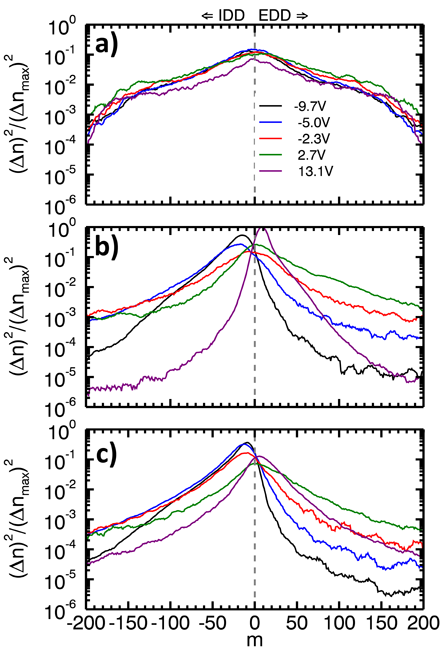
\includegraphics[width=8.5cm]{m_spec_regions_lab}}% made using plot_m_spec_amplitude_vs_frequency.pro
\caption{\label{fig:m_spec_regions} Azimuthal mode number m spectra for (a)core, (b)transition, and (c)edge regions for various bias states}
\end{figure}

Returning to the wavenumber/M-number spectra, a plot of the total power for each M-number is shown in Figure~\ref{fig:m_spec_regions}.  From this plot, it can be seen that the peak mode number in the unbiased edge regions is about m=15. At the limiter edge, this corresponds to a wavenumber of $k = m/r = 0.577 \text{cm}^{-1}$ or a wavelength of $\lambda = 10.9$cm. In the strongly biased regime, the peak switches to m=10 in the EDD direction which is $k = 0.384$ or $\lambda = 16.3$cm at the limiter edge. Since the growth of the coherent mode is strongest at the limiter edge, its is likely that these modes generate the peak at m=10.

\section{Comparison to a Linear Fluid Model}

To elucidate the contribution among mode types in the LAPD turbulence, it is useful to compare to results to a Braginskii fluid model which attempts to closely represent the collisional LAPD plasma. The following section discusses comparison between linear growth rates as calculated from a linearized set of Braginskii fluid equations with the fluctuation amplitudes as measured experimentally. While there is obvious interpretive difficulty in attempting to match saturated turbulent fluctuation amplitude with calculated growth rates of linear modes, any connects observed can be used to in concert with many experimental observations to get an idea of what physical processes may be at work. 

The basic Brakinskii fluid equations combine the density, ion momentum and electron momentum and charge conservation equation with collisional damping amongst ions, electrons and neutrals included:

\begin{gather}
\frac{\partial}{\partial t}(N) + (\textbf{v}_e \cdot \nabla)N = 0\\
Nm_e(\frac{\partial}{\partial t}(\textbf{v}_e)+(\textbf{v}_e \cdot \nabla)\textbf{v}_e) = -\nabla(Nk_bT_e) -Ne\left(\textbf{E}+ \frac{\textbf{v}_e}{c} \times \textbf{B}\right)-Nm_e\nu_{ei}(\textbf{v}_e-\textbf{v}_i)-Nm_e\nu_{en}\textbf{v}_e\\
Nm_i(\frac{\partial}{\partial t}(\textbf{v}_i)+(\textbf{v}_i \cdot \nabla)\textbf{v}_i) = -Ne\left(\textbf{E}+ \frac{\textbf{v}_i}{c} \times \textbf{B}\right)-Nm_i\nu_{in}\textbf{v}_i\\
\nabla \cdot \left(eN(\textbf{v}_{i\parallel}-\textbf{v}_{e\parallel})+eN(\textbf{v}_{i\perp}-\textbf{v}_{e\perp})\right) = 0
\label{eq:Braginskii}
\end{gather}

The following equations are a modified set of Braginskii fluid equations---augmented by the inclusion of radial density diffusion and ion-ion viscosity---used in an eigenmode solver code to calculate the growth rates and associated radially eigenfunctions of the modes present. 

\begin{gather}
\frac{\partial}{\partial t}(N) = -\textbf{v}_{\textbf{E}} \cdot \nabla N - \frac{\partial}{\partial z}(v_{\parallel e}N) - D_{n}\nabla^{2}_{\perp}N\\
\frac{\partial}{\partial t}(v_{\parallel e}) = -\textbf{v}_{\textbf{E}} \cdot \nabla v_{\parallel e} - \frac{m_{i}}{m_{e}} \frac{T_{e0}}{N_{0}}\frac{\partial}{\partial z}(N)-\frac{m_i}{m_e} \frac{\partial}{\partial z}(\phi) +1.71\frac{m_i}{m_e} \frac{\partial}{\partial z}(T_{e})-\nu_{e}v_{\parallel e}\\
\frac{\partial}{\partial t}(\varpi) = -\textbf{v}_{\textbf{E}} \cdot \nabla\varpi - \frac{\partial}{\partial z}(v_{\parallel e}N) + b\times \nabla N \cdot \frac{\nabla^{2}v_{E}}{2} - \nu_{in}\varpi -\mu_{ii}\nabla^{2}_{\perp}\varpi
\label{eq:eigsolver_eqns}
\end{gather}

where $\varpi = \nabla_{\perp} \cdot (N\nabla_{\perp}\phi)$ is the definition of vorticity. Cast in cylindrical geometry, with $\textbf{x} = (r,\theta,z)$, the solutions of the form

\begin{equation}
f(\textbf{x}) = f(r)exp(im_{\theta}\theta+ik_{\parallel}z-i\omega t)
\label{eq:eigenmode_func}
\end{equation}

are sought for density, N, parallel electron flow, $v_{\parallel e}$, and vorticity, $\varpi$, where $m_{\theta}$ is the azimuthal mode number and $k_{\parallel}$ is the axial wavelength which can be case in terms of an axial eigenvalue, $n_{z}$.

The origins of the three different instabilities can be highlighted from the many various terms in Equations~\ref{eq:eigsolver_eqns}. First the growth of resistive drift-waves can be narrowed down to the following subset of equations, 
%
\begin{gather}
\frac{\partial}{\partial t}(N) = -\textbf{v}_{\textbf{E}} \cdot \nabla N - \frac{\partial}{\partial z}(v_{\parallel e}N)\\
\frac{\partial}{\partial t}(v_{\parallel e}) = -\textbf{v}_{\textbf{E}} \cdot \nabla v_{\parallel e} - \frac{m_{i}}{m_{e}} \frac{T_{e0}}{N_{0}}\frac{\partial}{\partial z}(N)-\frac{m_i}{m_e} \frac{\partial}{\partial z}(\phi) -\nu_{e}v_{\parallel e}\\
\frac{\partial}{\partial t}(\varpi) = - \frac{\partial}{\partial z}(v_{\parallel e}N)
\label{eq:eigsolver_DWeqns}
\end{gather}
%
which highlight the DW drive dependence on the gradient in density as well as the parallel electron response. In order for the DW to be unstable, a phase shift between the density and plasma potential is necessary and in these equations is provided by the resistivity due to electron collisions (found in the term $\nu_{e}v_{\parallel e}$).

Similarly, the origin of rotational interchange is contained in the subset,
%
\begin{gather}
\frac{\partial}{\partial t}(N) = -\textbf{v}_{\textbf{E}} \cdot \nabla N\\
\frac{\partial}{\partial t}(\varpi) = -\textbf{v}_{\textbf{E}} \cdot \nabla\varpi + b\times \nabla N \cdot \frac{\nabla^{2}v_{E}}{2} - \nu_{in}\varpi
\label{eq:eigsolver_RIeqns}
\end{gather}
%
where the $b\times \nabla N \cdot \frac{\nabla^{2}v_{E}}{2}$ terms serves as the centrifugal force terms which initiates the mixing inherent in the interchange instability.

Lastly, the KH modes arise due to the gradient in the vorticity as in,
%
\begin{equation}
\frac{\partial}{\partial t}(\varpi) = -\textbf{v}_{\textbf{E}} \cdot \nabla\varpi
\label{eq:eigsolver_KHeqn}
\end{equation}
%
The remaining terms represent dissipative effects including perpendicular diffusion contained in the term $D_{n}\nabla^{2}_{\perp}N$, where $D_{n}$ taken to be classical diffusion in the code, and damping due to ion-ion viscosity contained in the term $\mu_{ii}\nabla^{2}_{\perp}\varpi$.

Of course, in the full set of equations coupling can take place between modes (e.g. drift-interchange modes). However, it should be noted that drift waves can only occur when a parallel wavelength is present; in other words, when there is a non-zero parallel eigennumber, n. For n=0, only rotational interchange and Kelvin-Helmholtz modes can be active. For comparisons to these experiments, only values of $n_{z} = $0 and 0.5 are used which correspond to infinite wavelength flute-like modes for $n_{z} = 0$ and wavelengths of the order of twice the machine length ($n_{z} = 0.5$), similar to the fundamental mode of a column with one open boundary condition and one closed boundary condition.

Using experimental profiles of density, temperature, and plasma potential for a given bias, Equations~\ref{eq:eigsolver_eqns} are solved as an algebraic eigenvalue problem for each azimuthal eigenmode number, m, and parallel eigenmode number, n. The range of m numbers used for this analysis was $m=1-80$ while n=0 or 0.5 as mentioned previously. The solutions consist of radial eigenfunctions for density, parallel velocity, and plasma potential of the form in Equation~\ref{eq:eigenmode_func} coupled with a growth rate, $\gamma$, and a frequency, $\omega = 2\pi f$. A positive(negative) growth rate indicates an unstable(stable) mode while the sign of the frequency indicates the propagation direction of the mode. For this analysis, only the density eigenfunctions, growth rates and frequencies were used.

Figure~\ref{fig:growth_freq_vs_mnum} shows typical results from the profiles of four different biases(Bias\#/(Limiter-Anode) potential : (a) Bias 1/-9.7V representing the unbiased IDD flow state, (b)Bias 8/-4.1V representing the zero flow state, (c)Bias 20/3.7V represented the moderate EDD flow state and (d)Bias 27/13.1V representing the strong EDD flow state. The growth rate and mode number for the fastest growing mode for each m-number is shown with the blue curves indicating calculations for n=0 and green for n=0.5. The mode selected is restricted to have a peak in its corresponding density eigenfunction within the a certain radial range; here, the modes are selected to be within radii of 20 and 32cm. If the fastest growing mode does not have a peak in its eigenfunction within the selected range, the next fastest growing mode is chosen and so on until all the possible modes are exhausted. This procedure ensures comparison to modes driven by the experimentally relevant gradients and not due to numerical artifacts.

The variations amongst the four biases shown demonstrate how the linear growth of instabilities are modified by the changes in the plasma profiles. In general, the n=0 modes appear to dominate the growth when both are present, certainly at lower m numbers. The exceptions are for small regions in the unbiased case and for m numbers larger than 20 in the moderate EDD flow case. In the zero flow case, only drift-waves can be active so only n=0.5 modes will be unstable. The portions of Figure~\ref{fig:growth_freq_vs_mnum} which show the frequency of the corresponding growing mode indicate the direction of propagation of the modes. In the unbiased case, the n=0 modes propagate in the positive direction which given the experimental arrangement corresponds to the IDD direction. In the EDD flow biases, the frequency sign is now negative indicating propagation in the EDD direction. In the highest bias shown, the frequencies are in the EDD for all m numbers suggesting that all of these modes are predominately interchange driven modes. The moderate EDD mode has frequencies in both directions. The lower m number modes are likely rotational interchange, but the higher m number modes can either be interchange modes driven by flow in the IDD (which does occur in the very far radial end of this bias) or are KH modes which do not have to propagate in the direction of the flow. The zero flow state with only drift waves shows that drift-waves propagate only in the EDD. 

\begin{figure}[!htbp]
\centerline{
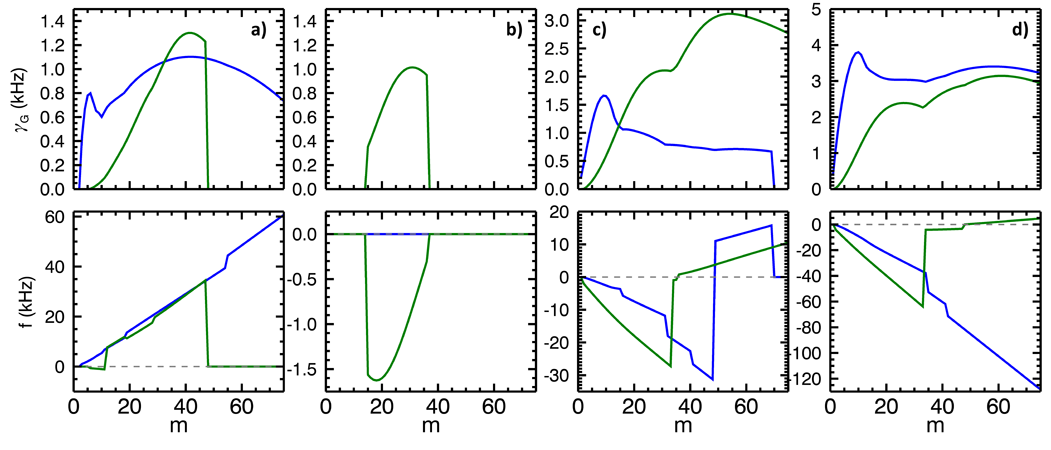
\includegraphics[width=8.5cm]{growth_freq_vs_mnum_lab}}%made with plot_fgm_vs_mnumber.pro (in eigsolver folder)
\caption{\label{fig:growth_freq_vs_mnum} Plots of the linear calculated growth rate and frequency of the fastest growing mode for each m number. Blue curves represent calculations using n=0. Green curves represent calculations with n=0.5. Column(a) shows calculations for Bias 1, (b) for Bias 8, (c) for Bias 20 and (d)for Bias 27.}
\end{figure}

In order to facilitate comparisons to the experimental spectral density functions, a ``growth rate density'' function is constructed using the eigenfunctions, growth rates and frequencies of the Braginskii equation solutions. First, the normalized eigenfunction of the fastest growing mode for each m number is scaled to the value of the growth rate to create a localized growth function---that is, the strength of the growing mode is maximum at the peak of the eigenfunction and reduced accordingly away from the peak. This radial distribution of growth rate is broken into wavenumbers, $k$, given the m number and radius. Connected to each value of k is the frequency of the mode, and the sign of the frequency is converted into a sign of the wavenumber. Then, this collection of signed wavenumbers or frequencies is histogrammed into wavenumber and frequency bins and then averaged according to the histogram count. What results is a contour of average growth rate as a function of wavenumber and frequency which can then be compared directly to the spectral density functions from experiment.

\begin{figure}[!htbp]
\centerline{
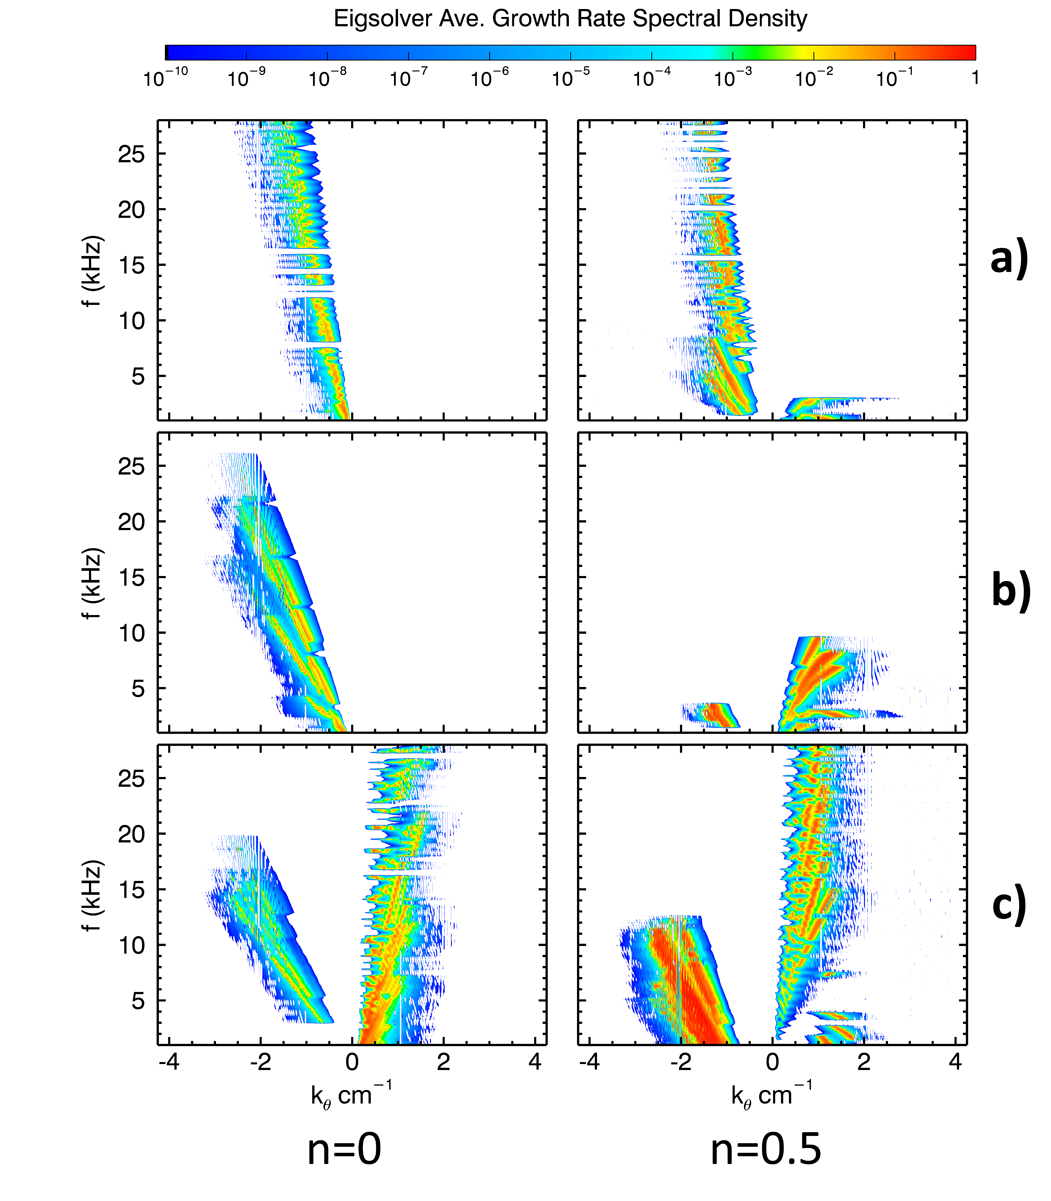
\includegraphics[width=8.5cm]{growth_density_20to32_lab}}% made using plot_eigsolver_kperp_spectral_density_biasRegions.pro
\caption{\label{fig:growth_density_20to32} Growth Density functions from linear eigensolver calculations for 3 bias groupings: (a)Bias0-9, (b)Bias 10-14, and (c)Bias 15-29. Growth rates were restricted to the radial region of 20 to 32cm.}
\end{figure}

Figure~\ref{fig:growth_density_20to32} shows the ``growth'' density functions created using the same data presented in Figure~\ref{fig:growth_freq_vs_mnum} separated into different bias groupings and parallel eigenvalue n. The growth density functions shown were averaged for three bias regions: Row (a)Bias 0-9 representing all the biases with flow in the IDD; (b)Bias 10-14 representing the region near zero flow and just into the EDD flow; and (c)Bias 15-29 representing moderate to strong EDD flow. The first column shows these growth density functions calculated for n=0 and the second for n=0.5. The negative signed wavenumbers indicate mode propagation in the IDD while positive signed wavenumbers indicate EDD. The features of these plots will be explored in more detail when being compared to experimental data.

\section{Conclusions}

The authors would like to thank Zoltan Lucky and Marvin Drandell for their valuable technical support.  This work
was supported by the National Science Foundation (PHY-0903913) and performed using the Basic Plasma Science Facility at UCLA. The BaPSF is funded by the
Department of Energy and NSF.

\providecommand{\noopsort}[1]{}\providecommand{\singleletter}[1]{#1}%
\begin{thebibliography}{10}

%shearing theory
\bibitem{burrell97}
K. Burrell, Phys. Plasmas {\bf 4},  1499  (1997).

\bibitem{burrell99}
K. Burrell, Phys. Plasmas {\bf 6},  4418  (1999).

\bibitem{terry00}
P. Terry, Rev. Mod. Phys. {\bf 72},  109  (2000).

\bibitem{oost03}
G. Van Oost , J. Adamek and V. Antoni, P. Balan, J.A. Boedo, P. Devynck, I. Duran, L. Eliseev, J.P. Gunn, M. Hron, C. Ionita, S. Jachmich, G.S. Kirnev, E. Martines, A. Melnikov, R. Schrittwieser, C. Silva, J. Stockel, M. Tendler, C. Varandas, M. Van Schoor, V. Vershkov and R.R. Weynants, Plas. Phys. Control Fusion {\bf 48}, 621 (2003).

\bibitem{sakai93}
O. Sakai, Y. Yasaka and R. Itatani, Phys. Rev. Lett. {\bf 70},  4071 (1993).

\bibitem{maggs07}
J.E. Maggs, T.A. Carter and R.J. Taylor, Phys. Plasmas {\bf 14},  052507  (2007).

\bibitem{carter09}
T.A. Carter and J.E. Maggs, Phys. Plasmas {\bf 16},  012304  (2009).

\bibitem{schaffner12}
D.A. Schaffner, T.A. Carter, G.D. Rossi, D.S. Guice, J.E. Maggs, S.Vincena and B. Friedman, Phys. Rev. Lett. {\bf 109}, 135002 (2012).

\bibitem{burrell92}
K.H. Burrell, T.N. Carlstrom, E.J. Doyle, D. Finkenthal, P. Gohil, R.J. Groebner, D.L. Hillis, J. Kim, H. Matsumoto, R.A. Moyer, T.H. Osborne, C.L. Rettig, W.A. Peebles, T.L. Rhodes, H. St.John, R.D. Stambaugh, M.R. Wade and J.G. Watkins, Plas. Phys. Control Fusion {\bf 34}, 1859 (1992). 

\bibitem{wagner07}
F. Wagner, Plas. Phys. Control Fusion {\bf 49}, B1 (2007).

\bibitem{taylor89}
R.J. Taylor, M.L. Brown, B.D. Fried, H. Grote, J.R. Liberati, G.J. Morales, P. Pribyl, D. Darrow and M. Ono, Phys. Rev. Lett. {\bf 63},  2365  (1989).

\bibitem{weynants92}
R.R. Weynants, G. Van Oost, G. Bertschinger, J. Boedo, P. Brys, T. Delvigne, K.H. Dippel, F. Durodie, H. Euringer, K.H. Finken, D.S. Gray, J.D. Hey, D.L. Hillis, J.T. Hogan, L. Konan, R. Leners, A.M. Messian, A. Pospieszczyck, U. Samm, R.P. Schorn, B. Schweer, G. Telesca, R. Vannieuwenhove and P.E Vandenplas, Nucl. Fusion {\bf 32},  837  (1992).

\bibitem{weynants98}
R.R. Weynants, S. Jachmich and G. Van Oost, Plas. Phys. Control Fusion {\bf 40}, 635 (1998).

\bibitem{boedo00}
J. Boedo, D. Gray, S. Jachmich, R. Conn, G.P. Terry, G. Tynan, G. Van Oost, R.R. Weynants and TEXTOR Team, Nucl. Fusion {\bf 40},  7  (2000).

\bibitem{boedo02}
J.A. Boedo, D.S. Gray, P.W.Terry, S. Jachmich, G.R. Tynan, R.W. Conn and TEXTOR-94 Team, Nucl. Fusion, {\bf 42}, 117 (2002).

\bibitem{biglari90}
H. Biglari, P.H. Diamond and P.W. Terry, Phys. Fluids B. {\bf 2},  1  (1990).

\bibitem{shaing90}
K.C. Shaing, E.C. Crume and W.A. Houlberg, Phys. Fluids B {\bf 2}, 6 (1990).

\bibitem{zhang92}
Y.Z. Zhang and S.M. Mahajan, Phys. Fluids B {\bf 4}, 1385 (1992).

\bibitem{zhang93}
Y.Z. Zhang and S.M. Mahajan, Phys. Fluids B {\bf 5}, 7 (1993).

\bibitem{ware96}
A.S. Ware, P.W. Terry, P.H. Diamond and B.A. Carreras, Plasma Phys. Control Fusion {\bf 38},  1343  (1996).

\bibitem{ware98}
A.S. Ware, P.W. Terry, B.A. Carreras and P.H. Diamond, Phys. Plasmas {\bf 5}, 173 (1998).

\bibitem{terry01}
P.W. Terry, D.E. Newman and A.S. Ware, Phys. Rev. Lett. {\bf 87}, 185001  (2001).

\bibitem{kim03}
E.-J. Kim and P.H. Diamond, Phys. Rev. Lett. {\bf 90}, 7 (2003).

\bibitem{kim04}
E.-J. Kim, P.H. Diamond and T.S. Hahm, Phys. Plasmas {\bf 11},  10  (2004).

\bibitem{newton11}
A.P.L. Newton and E.-J. Kim, Phys. Plasmas {\bf 18}, 052305 (2011).

\bibitem{gek91}
W. Gekelman, H. Pfister, Z. Lucky, J. Bamber, D. Leneman and J. Maggs, Rev. Sci. Instrum. {\bf 62},  2875  (1991).

\bibitem{hahm94}
T.S. Hahm, Phys. Plasmas {\bf 1}, 2940 (1994).

\bibitem{leconte06}
M. Leconte, P. Beyer, S. Benkadda and X.Garbet, Phys. Plasmas {\bf 13} 112301 (2006).

\bibitem{newton07}
A.P.L. Newton and E.-J. Kim, Phys. Plasmas {\bf 14}, 122306 (2007).

\bibitem{terry06}
P.W. Terry and R. Gatto, Phys. Plasmas {\bf 13}, 062309 (2006).

\bibitem{staebler13}
G.M. Staebler, R.E. Waltz, J. Candy and J.E. Kinsey, Phys. Rev. Lett. {\bf 110}, 055003, (2013)).

\bibitem{friedman12}
B. Friedman, T.A. Carter, M.V. Umansky, D. Schaffner and B. Dudson, Phys. Plasmas {\bf 19}, 102307 (2012).

\bibitem{umansky11}
M. Umansky {\it et~al.}, Phys. Plasmas {\bf 18},  055709  (2011).

\bibitem{popovich10BOUT}
P.Popovich, M.V. Umansky, T.A. Carter and B. Friedman, Phys. Plasmas {\bf 17}, 122312 (2010).

\end{thebibliography}
\end{document}
